\section{Vollständigkeit}
\subsection{???}
Supremumseigenschaft zeichnet $ \R $ aus.\\
Cauchy-Folgen\\
In $ \R $ sind Cauchy-Folgen und konvergente Folgen gleich, in $ \Q $ z.B. nicht.\\
Cauchy-Folgen sind beschränkt\\
es ist nicht so, dass alle Beschränkte Folgen, Cauchy-Folgen sind\\
\begin{subdefinition}[Cauchyfolge]
	Eine reele Folge $(a_n)$ heißt \textbf{Cauchy} oder \textbf{Cauchyfolge}, falls für alle $\varepsilon > 0 $ ein $ N \in \N $ existiert, sodass $ |a_n - a_m| < \varepsilon $ für allle $ n, m \geq N $.
	\fbox{$\forall \varepsilon > 0 \exists N \in \N: \forall n, m \geq N : | a_n - a_m| < \varepsilon $}
\end{subdefinition}

\begin{subtheorem}
	Sei $ (a_n) $ eine folge in $ \R $. Dann gilt:
	\begin{enumerate}[label=(\roman*)]
		\item Ist $ (a_n) $ konvergent, so ist $ (a_n) $-Cauchy.
		\item Ist $ (a_n) $ Cauchy, dann ist $ (a_n) $ beschränkt.
		\item Ist $ (a_n) $ konvergent, so ist $ (a_n) $ beschränkt.
	\end{enumerate}
	\begin{subproof*}
		\begin{enumerate}[label=(\roman*)]
			\item Sei $ \varepsilon 0 $ beliebig. Da $ (a_n) $ konvergent, existiert ein $ a \in \R $ und ein $ N \in \N $ mit $ |a_n - a| < \frac{\varepsilon}{2} $.\\
				Seien $ n, m \in \N $, dann gilt
				\[ | a_n - a_m| = | (a_n - a) + (a- a_m)| \leq |a_n - a| + |a - a_m| < \frac{\varepsilon}{2} + \frac{\varepsilon}{2} = \varepsilon \]
			\item Setze $ \varepsilon = 1 $. Dann finden wir ein $ N \in \N $ mit $ |a_n - a_m| < 1 $ für alle $ n, m \geq N $.\\
				Die Menge $ \{ |a_1|,\dotsc, |a_N| \} $ ist endlich, hat also ein Maximum, nenne dieses $ M $.\\
				Für alle $ n \geq \N $ gilt also $ |a_n| \leq M $ falls $ 1 \leq n \leq M $,
				\[ |a_n| \leq |a_n - a_N| + a_N| \leq |a_n - a_N| + |a_N| \leq 1 + M \text{ falls } n \geq N \]
				Deswegen ist $ (a_n) $ durch $ 1 + M $ beschränkt.
			\item Direkt aus (i) und (iii)
		\end{enumerate}
	\end{subproof*}
\end{subtheorem}
\begin{subexample}[Beschränktheit und nicht Cauchy]
	Betrachte $ (a_n) \coloneqq (-1)^n $. Dann ist $ |a_n| = 1 $ für alle $ n \in \N $ und speziell $ (a_n) $ beschränkt. Wähle $ 0 < \varepsilon < 2 $. Dann gilt für bel $ N \in \N $
	\[ |a_n - a_{n+1}| = 2 > \varepsilon \]
\end{subexample}

\subsection{Teilfolgen undn der Satz von Bolzano-Weierstraß}
\begin{itemize}
	\item \[ ( ( -1 )^n ) : \begin{cases} \text{gerade Folgeglieder: immer $-1$}\\\text{ungerade Folgeglieder: immer $-1$} \end{cases} \]
\end{itemize}

\begin{subdefinition}
	Sei $ (a_n) \subset \R $ Folge und $ n : \N \to \N $ eine monoton wachsende Abbildung. Dann heißt $ (a_{n(k)}) $ \textbf{Teilfolge}
\end{subdefinition}

\begin{subexample}
	$(a_n) = ( (-1)^n ) $
	\begin{itemize}
		\item $ n(k) = 2k \rightsquigarrow (a_{n_k})$ = Teilfolge der geraden Folgenglieder
		\item $ n(k) = 2k - 1 \rightsquigarrow (a_{n_k})$ = Teilfolge der ungeraden Folgenglieder
	\end{itemize}
\end{subexample}

\begin{subdefinition}
	Sei $ (a_n) \subset \R $ und $ (a_{n_k}) \subset (a_n) $ Teilfolge die gegen $ a \in \R $ konvergiert. Dann heißt $ a $ \textbf{Häufungspunkt} von $ (a_n) $. Wir definieren dann den \textbf{Limes superior} via
	\[\limsup_{n\to\infty} \coloneqq \inf_{n\in\N} \sup_{k\geq n} a_k, \]
	und den \textbf{Limes inferior} via
	\[ \liminf_{n\to\infty} a_n \coloneqq \sup_{n\in\N} \inf_{k\geq n} a_k. \]
	\begin{itemize}
		\item $ a $ HP von $ (a_n)  \iff \forall \varepsilon > 0 \forall N \in \N \exists n \geq N : | a_n - < | < \varepsilon $.
	\end{itemize}
\end{subdefinition}

\begin{subexample}
	$ (a_n) = (a) $ für $ a \in \R $ (konstante Folge), so $ a $ einzelner Häufungspunkt; allgemeiner: Falls $ a_n \to a $ konvergiert,  so ist a einzelner Häufungspunkt.
\end{subexample}

\begin{subexample}
	$ (a_n) = (-1)^n $, so sind $ +1 $ und $ -1 $ Häufungspunkte der Folge. Weiter $ \limsup_{n\to\infty} a_n = +1 $ und $ \liminf_{n\to\infty} a_n = -1 $.\\
	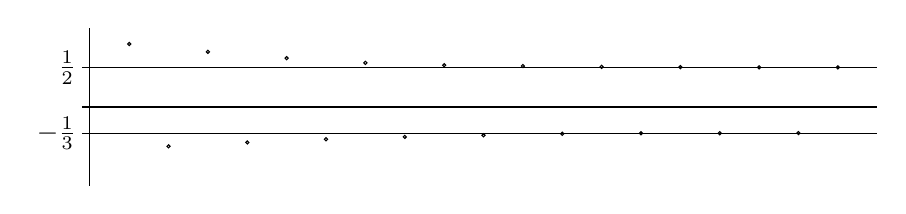
\begin{tikzpicture}
		\draw (0, -1) -- (0, 1);
		\draw (-0.1, 0) -- (10, 0);
		\draw[thin] (-0.1, 0.5) -- (10, 0.5);
		\draw[thin] (-0.1, -0.333) -- (10, -0.333);
		\draw (-0.05, -0.333) node[anchor = east] {$-\frac{1}{3}$} -- (0.05, -0.333);
		\draw (-0.05, 0.5) node[anchor = east] {$\frac{1}{2}$} -- (0.05, 0.5);
		\draw (0.5, 0.8) circle (0.02);
		\draw (1.5, 0.7) circle (0.02);
		\draw (2.5, 0.62) circle (0.02);
		\draw (3.5, 0.56) circle (0.02);
		\draw (4.5, 0.53) circle (0.02);
		\draw (5.5, 0.52) circle (0.02);
		\draw (6.5, 0.51) circle (0.02);
		\draw (7.5, 0.505) circle (0.02);
		\draw (8.5, 0.503) circle (0.02);
		\draw (9.5, 0.502) circle (0.02);
		\draw (1, -0.5) circle (0.02);
		\draw (2, -0.45) circle (0.02);
		\draw (3, -0.41) circle (0.02);
		\draw (4, -0.38) circle (0.02);
		\draw (5, -0.36) circle (0.02);
		\draw (6, -0.34) circle (0.02);
		\draw (7, -0.335) circle (0.02);
		\draw (8, -0.333) circle (0.02);
		\draw (9, -0.332) circle (0.02);
	\end{tikzpicture}
\end{subexample}

\begin{subtheorem}[Bolzano Weierstraß]
	Jede beschränkte Folge in $ \R $ besitzt eine konvergente Teilfolge.
\end{subtheorem}
\begin{sublemma}
	Jede Folge in $\R$ hat eine monotone Teilfolge.
\end{sublemma}
\begin{subproof*}
	Sei $ (a_n) \subset \R $ beschränkt. Nach Lem \ref{4.2.7} gibt es eine monotone Teilfolge, die natürlich auch beschränkt ist. Nach dem Satz über monotone, beschränkte Folgen konvergiert diese Teilfolge.\qed
\end{subproof*}
Brauchen:
\begin{subproof*}
	Sei $ (a_n) \subset \R $ bel. Wir nennen $ a_{n_0} (n_0 \in \N)$ \textbf{Gipfelpunkt}, falls:
	\begin{enumerate}[label=(\roman*)]
		\item \textbf{unendlich viele Gipfelpunkte}: Sei dann $ (a_{n_k}) $ Teilfolge der Gipfelpunkte.
			Dann \[ n_1 \leq n_2 \leq n_3 \leq \dotsb \text{ und} \]
			\[ a_{n_1} \geq a_{n_2} \geq a_{n_3} \geq \dotsb \]
			Also ist $ (a_{n_k}) $ monoton fallend.
		\item \textbf{endlich viele oder keine Gipfelpunkte:} Hier existiert
			\[ N \in \N : n \geq N \implies a_n \] kein Gipfelpunkt. Also gilt nicht:
			D. h. $ \exists n_1 \geq N: a_N < a_{n_1} \implies a_{n_1} $ kein Gipfelpunkt $\implies \exists N_2 \gneqq n_1 : a_{n_1} < a_{n_2}$, usf. Dann ist $ (a_{n_k} ) $ monoton wachsend.\qed
	\end{enumerate}
\end{subproof*}

\subsection{Charakterisierung der Vollständigkeit}
Für $ a \leq b $ sei $ [a, b] \coloneqq \{ x \in \R : a \leq x \leq b \} $. Der Durchmesser von $ [ a, b ] : \operatorname{diam}([a, b]) = b - a $

\begin{sublemma}
	Sei $ (a_n) $ Cauchyfolge, die eine gegen $ a\in \R $ konvergiente Teilfolge besitzt. Dann konvergiert $ (a_n ) $ gegen $ a $.
	\begin{subproof*}
		$\forall\varepsilon > 0 \exists N \in \N \forall n, m \geq N : | a_n - a_m | < \frac{\varepsilon}{2} $. Wähle zu $ \varepsilon > 0 $ ein solches $ N \in \N $.
		Dann gibt es wegen konvergenter Teilfolge einen Index $ \widetilde{N} \geq N : | a - a_{widetilde{N}} | < \frac{varepsilon}{2}$.
		Dann $ \forall n \geq N : $
		\begin{align*}
			| a_n - a | &= | ( a_n - a_{\widetilde{N}} ) + ( a_{\widetilde{N}} - a ) |\\
			&< \underbrace{a_n - a_{\widetilde{N}}|}_{\frac{\varepsilon}{2}} + \underbrace{a_{\widetilde{N}} - a|}_{\frac{\varepsilon}{2}} < \varepsilon
		\end{align*}
	\end{subproof*}
\end{sublemma}

\begin{subtheorem}
	Die folgenden Prinzipien sind auf $ \R $ äquivalent:
	\begin{enumerate}[label=(\roman*)]
		\item \textbf{Supremumseigenschaft:} Jede nichtleere, nach oben beschrenkte Menge hat ein Supremum.
		\item \textbf{Bolzano-Weierstraß-Eigenschaft:} Jede beschränkte Folge hat eine konvergente Teilfolge
		\item \textbf{Vollständigkeit:} Jede Cauchyfolge konvergiert
		\item \textbf{Intervallscachtelungsprinzip:} Sind $ (a_n), (b_n) \subset \R $ mit $ \forall n \in \N : a_n \leq b_n \wedge [a_{n+1}, b_{n+1}] \subset [a_n, b_n] $ mit
			$\lim_{n\to\infty} \operatorname{diam}([a_n, b_n]) = 0 $, so \textbf{existiert genau ein}
			\[ x \in \bigcap_{n\in\N}[a_n, b_n]. \]
	\end{enumerate}
	\begin{subproof*}
		Plan: $ (i) \implies (ii) \implies (iii) \implies (iv) \implies (i) $
		\begin{description}
			\item[Ad $ (i) \implies (ii) $] Die Supremumseigenschaft ist die einizige Zutat, um Bolzano-Wei\-er\-straß zu zeigen. Damit folgt $(ii)$ aus $(i)$
			\item[Ad $ (ii) \implies (iii) $] Sei $ (a_n) $ Cauchyfolge. Nach letzter Vorlesung ist $ ( a_n ) $ beschränkt, und nach $ (ii) $ hat $ (a_n ) $ also konvergiert Teilfolge. Nach Lem \ref{4.3.1} konvergiert dann aber bereits $ (a_n) \implies (iii) $
			\item[Ad $ (iii) \implies (iv)$] Sei $ ([a_n, b_n]) $ eine \textbf{Intervallschachtelung} mit $ \operatorname{diam}([a_n, b_n]) \to 0, n \to \infty. $. Sei $ \varepsilon > 0 $.
				Dann \[ \exists N \in \N : \forall n \geq N : \underbrace{\operatorname{diam}([a_n, b_n])}_{b_n - a_n} < \varepsilon \].
				Dann $ \forall n, m \geq N : a_m \in [a_n, b_n] $ (da Intervallschachtellung), also:
				\[ | a_n - a_m | \leq | a_n - b_n| < \varepsilon \implies (a_n) \textbf{ Cauchy}.\]
				Ähnlich: $ (b_n) \text{Cauchy} \overset{(iii)}{\implies} \exists a, b \in \R: a_n \to a, b_n \to b $.
				\[ | a- b| = \lim_{n\to\infty} \underbrace{|a_n -b_n}_{\operatorname{diam}([a_n, b_n])} = 0 \implies a = b. \]
				Kurz zu
				\[ a \in \bigcap_{n\in\N}[a_n, b_n] : (a_n) \text{ monoton wachsend}, (b_n) \text{ monoton fallend} \]
				\begin{align*}
					&\overset{\text{Stabilität der KG-Relation}}{\implies}
					\begin{drcases}
						a_1 \leq a_2 \leq \dotsb \leq a\\
						b  \geq \dotsb \geq b_2 \geq b_1
					\end{drcases}\\
					&\implies a_1 \leq a_2 \leq \dotsb \leq a = b \leq \dotsb \leq b_2 \leq b
				\end{align*}
				hier fehlt noch was ...
		\end{description}
	\end{subproof*}
	\begin{subproof-headless}
		\begin{description}
			\item[Ad $(iv) \implies (i)$] Sei $ A \subset \R $ nichtleer und nach oben beschränkt. Zu zeigen $ A $ besitzt Supremum. Wähle $ x_0 \in A $, sowie $ y_0 \in \R $ eine obere Schranke von $ A $. Seien für $ n \in \N_0 $ die Intervalle $ [x_0, y_0], \dotsc, [x_n, y_n] $ definiert. Setzte dann
				\begin{align*}
					x_{n+1} &\coloneqq%
					\begin{cases}%
						x_n, & \text{falls } [\frac{x_n+y_n}{2}, y_n] \cap A \neq \emptyset\\
						\xi \in [\frac{x_n + y_n}{2}, y_n] \cap A & \text{sonst}
					\end{cases}\\
					y_{n+1} &\coloneqq%
					\begin{cases}%
						\frac{x_n + y_n}{2}, & \text{falls } [\frac{x_n+y_n}{2}, y_n] \cap A \neq \emptyset\\
						y_n & \text{sonst}
					\end{cases}%
				\end{align*}
				\begin{itemize}
					\item $[x_{n+1}, y_{n+1}] \subset [x_n, y_n] : \%$ (sieht man ja)
					\item Beh.: $ | x_n - y_n | \leq 2^{-n} | x_0 - y_0 \forall n \in \N_0 $ (reference star)
					%\par\vspace{\textheight minus \textheight}\pagebreak
						\begin{description}
							\item[I.A.:] erfüllt.
							\item[I.S.:] $ n \curvearrowright n+1 $. Gelte (star) für ein $ n \in \N_0 $. Entweder
								\begin{enumerate}[label=(\alph*)]
									\item $ | x_{n+1} - y_{n+1} | = \left| x_n - \left( \frac{x_n + y_n}{2} \right) \right| = \frac{1}{2} | x_n - y_n | \overset{IV}{\leq} 2^{-(n+1)} |x_0 - y_0| $
									\item $ | x_{n+1} - y_{n+1} | = | \xi - y_n | = y_n - \xi \leq y_n - \frac{1}{2} (x_n + y_n) = \frac{1}{2} (x_n - y_n) \overset{IV}{\leq} 2^{-(n+1)} | x_0 - y_0 | $
								\end{enumerate}
						\end{description}
						$ \implies \operatorname{diam}([x_N, y_n]) \to 0, n \to \infty $. Nach $ (iv) \exists! x \in \bigcap_{n \in \N_0}[x_n, y_n] $. \textbf{Zeige nun:} $ x = \sup(A) $. \textbf{$x$ obere Schranke}. Hierzu: $ x = \lim_{n\to\infty} y_n $. Also $ \forall z \in A $:
						\[ z \overset{\forall n}{\leq} y_n \overset{n\to\infty}{\to} x \implies z \leq x \implies \text{ obere Schranke} \]
						\textbf{$x$ kleinste obere Schranke:}
						Angenommen es gäbe $ x^\prime \in \R, x^\prime \lneqq x \wedge x^\prime$ obere Schranke.
						Aber $ x_n \to x $ Aber $ \forall n \in \N_0 : x_n \in A$.
						Dann aber $ \exists N \in \N : \forall n \geq N : x^\prime < x_n < x $.
						(Wähle $ \varepsilon = \frac{1}{2} | x - x^\prime|) $).
						Widerspruch, da $ x^\prime $ keine obere Schranke. Also gilt (i)\qed
				\end{itemize}
		\end{description}
	\end{subproof-headless}
\end{subtheorem}

\begin{subexample*}[einfach Beispiel aus Vorlesung]
	Ich glaube das soll zeigen, dass irgendwas an $ \R $ besonders
	\[ [ \sqrt{2} - 1, \sqrt{2} + \frac{1}{n} ] \]
	\[ \sqrt{2} - \frac{2}{n} \leq a_n leq \sqrt{2} - \frac{1}{n} \]
	\[ \sqrt{2} + \frac{1}{n} \leq b_n leq \sqrt{2} + \frac{1}{n} \]
	\[ [ a_n, b_n ], a_n, b_n \in \Q \]
\end{subexample*}

